\chapter{Applicability of the Fisher Matrix}
\label{app:fisher_valid}

As established in Sec.~\ref{sec:fisher_prereq}, one requirement for the Fisher
Matrix to be valid is that the observables (\ie the bin counts for PINGU) are
described by linear functions of the parameters, hence the partial derivatives
entering (\ref{eqn:fisher_def}) can be considered to be constant within the
considered range. To quantify the non-linearity, one can define the quantity
\begin{equation}
 \Upsilon_n(p_i) = \left(N_n(p_{i,\,\mathrm{fid}} + \sigma_{p_i}) -
                          N_n(p_{i,\,\mathrm{fid}}) +
                     \frac{\partial N_n}{\partial p_i}\sigma_{p_i}\right)
                       \bigg/ N_n(p_{i,\,\mathrm{fid}}) \quad,
 \label{eqn:non-lin}
\end{equation}
describing the relative contribution of the non-linear terms to the variation
of the event count $N_b$ in bin $b$ as a function of the parameter $p_i$ over
its uncertainty range $p_{i,\,\mathrm{fid}} \pm \sigma_{p_i}$.

As one can see from Figs.~\ref{fig:nonlinearities1} and
\ref{fig:nonlinearities2}, for the simple scaling parameters like the mass
hierarchy $h$ or the overall normalisation $n_\aeff$ non-linearities are on the
order of the machine precision. But also for the physics parameters they are
typically smaller than $10^{-3}$, hence the requirement of linearity is well
fulfilled.

For means of illustration, the actual dependence of all bin entries on the
systematic parameters is shown as well. By eye, deviations from linearity can
only be recognised for \dm{31} and the energy scale. Since both shift the
sinusoidal oscillation pattern in energy non-linearities have to be expected,
however they only occur on a scale conceivably larger than the actual
uncertainty range.

\begin{figure}[p]
 \centering
 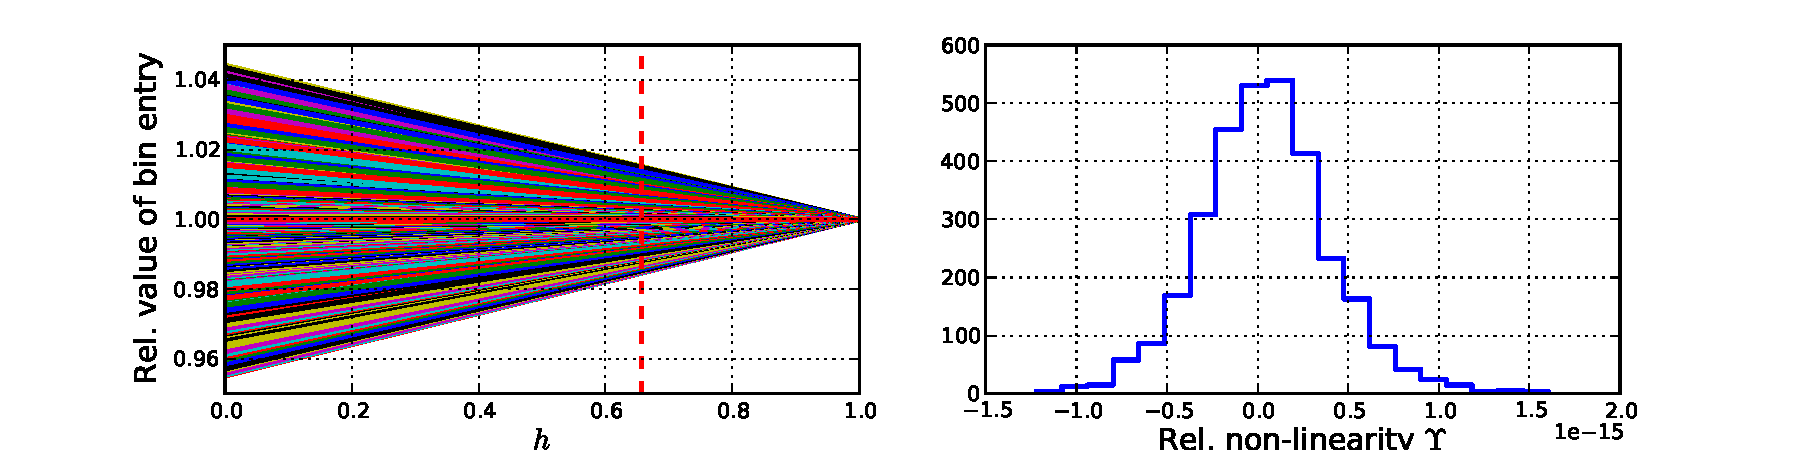
\includegraphics[width=\linewidth]{hierarchy}
 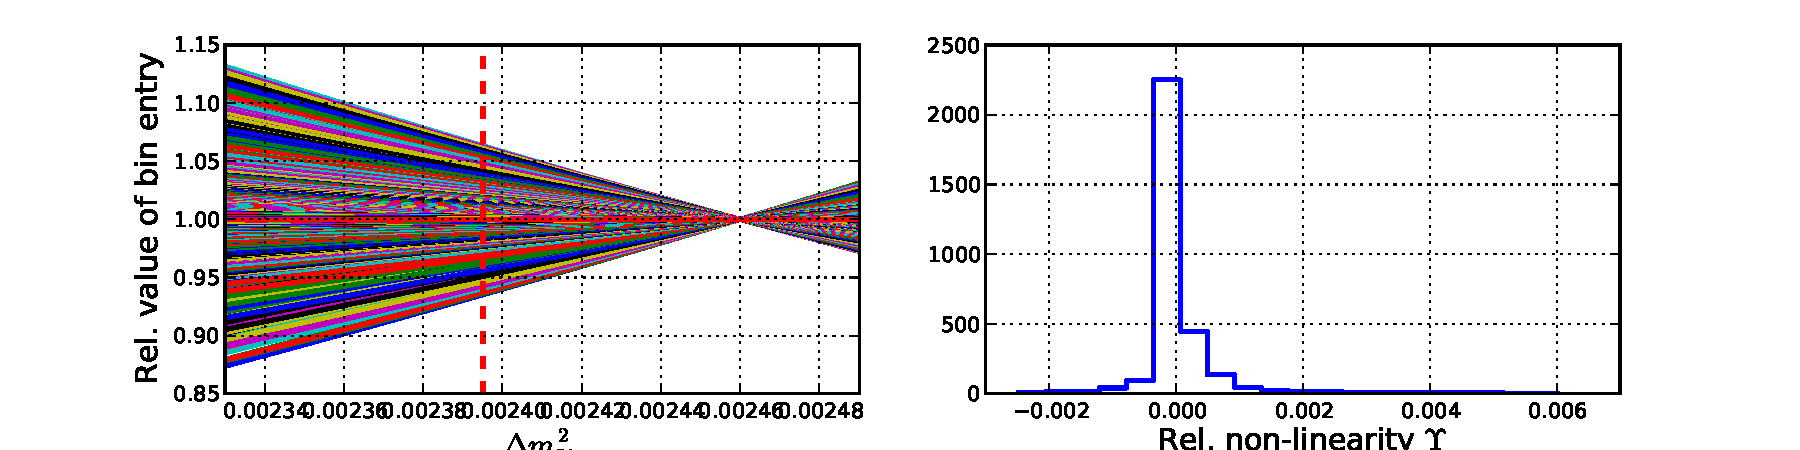
\includegraphics[width=\linewidth]{deltam31}
 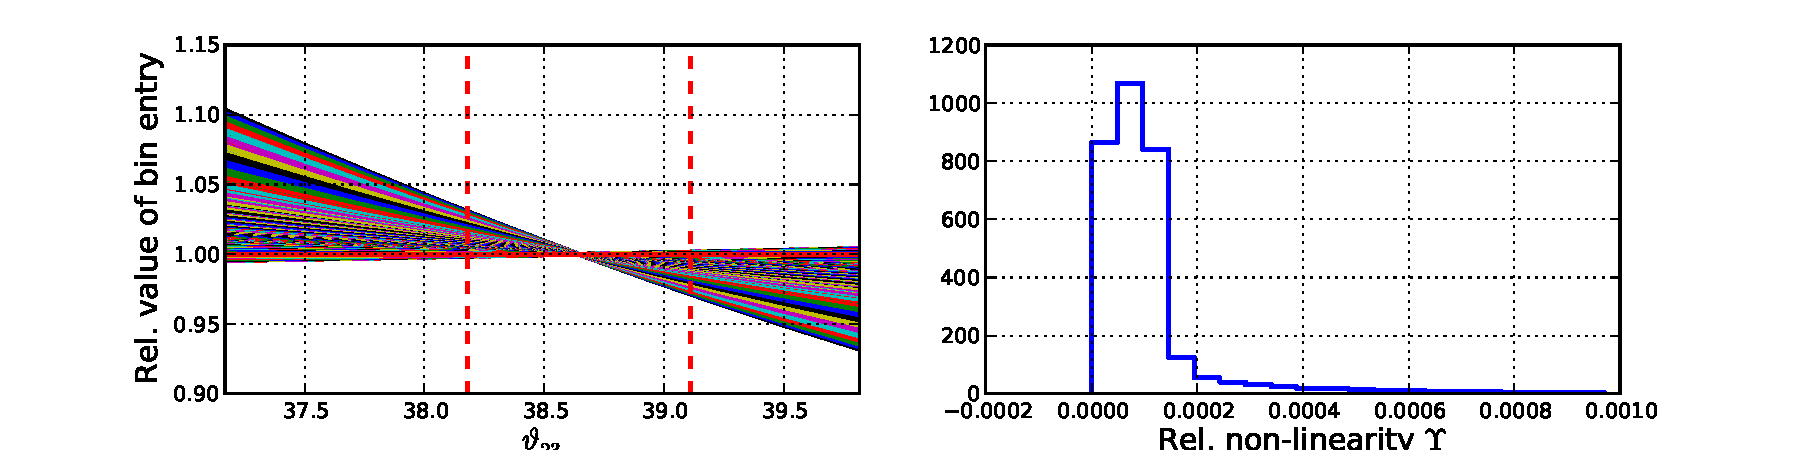
\includegraphics[width=\linewidth]{theta23}
 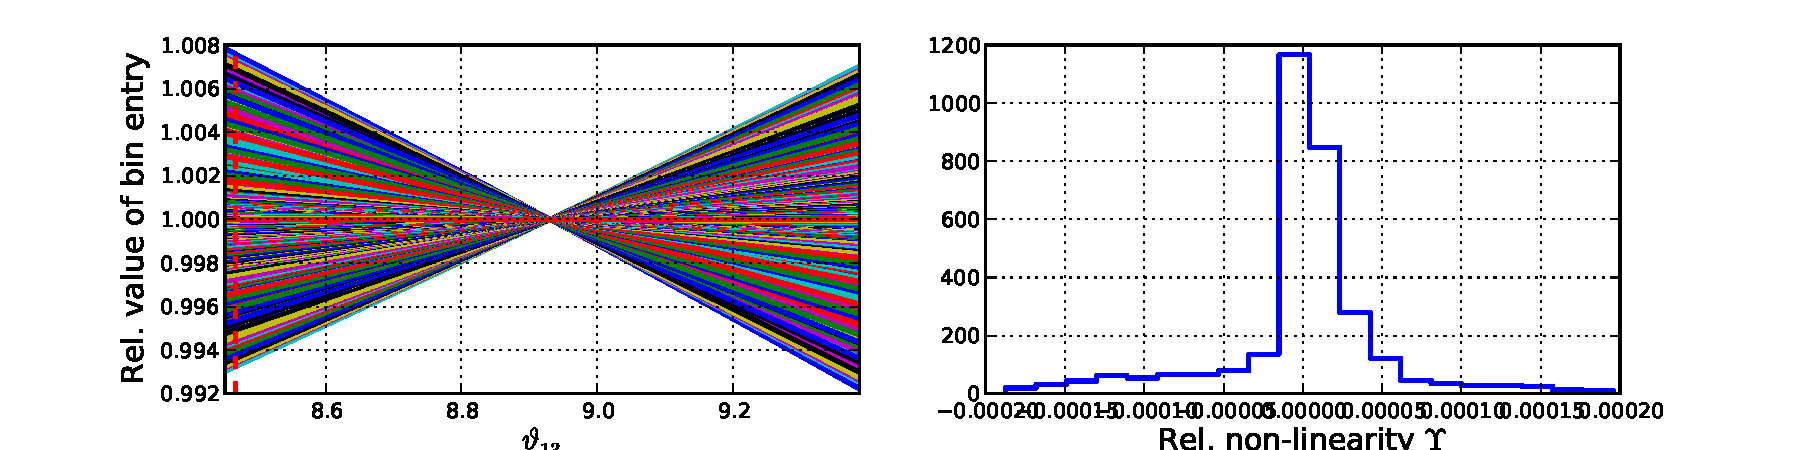
\includegraphics[width=\linewidth]{theta13}
 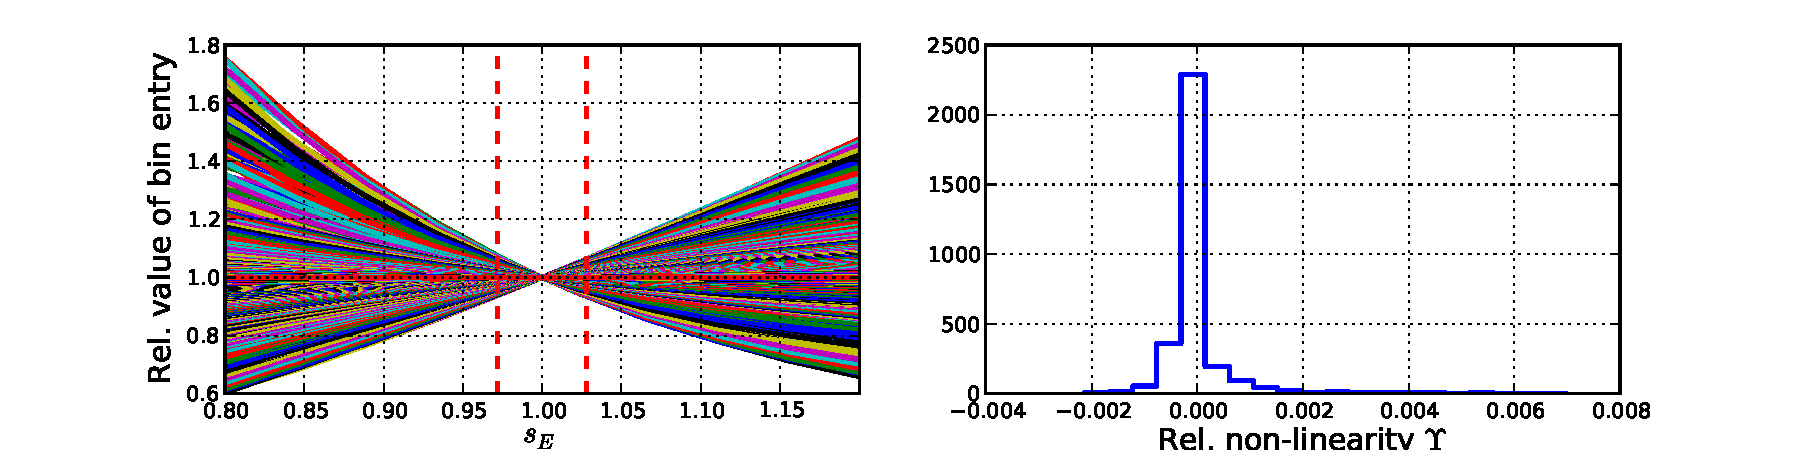
\includegraphics[width=\linewidth]{energy_scale}
 \caption{\emph{Left:} Relative values of all bin entries in the analysis
  histograms as functions of the systematic parameters. The the entries at the 
  fiducial parameter values are set to one. The vertical lines indicate the full
  error range as listed in Tab.~\ref{tab:baseline_results}. \\
  \emph{Right:} Histograms of the non-linearities $\Upsilon$ of the bin counts
  as functions of different systematic parameters (see equation
  (\ref{eqn:non-lin})).}
 \label{fig:nonlinearities1}
\end{figure}

\begin{figure}[p]
 \centering
 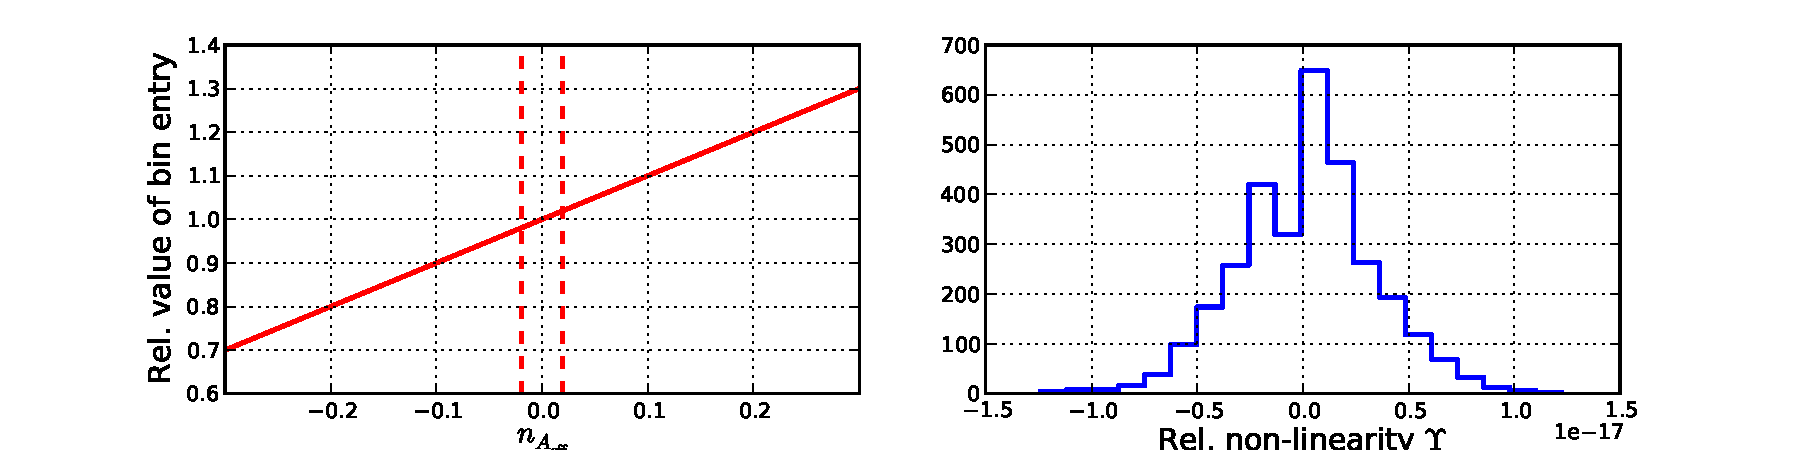
\includegraphics[width=\linewidth]{a_eff_scale_flat}
 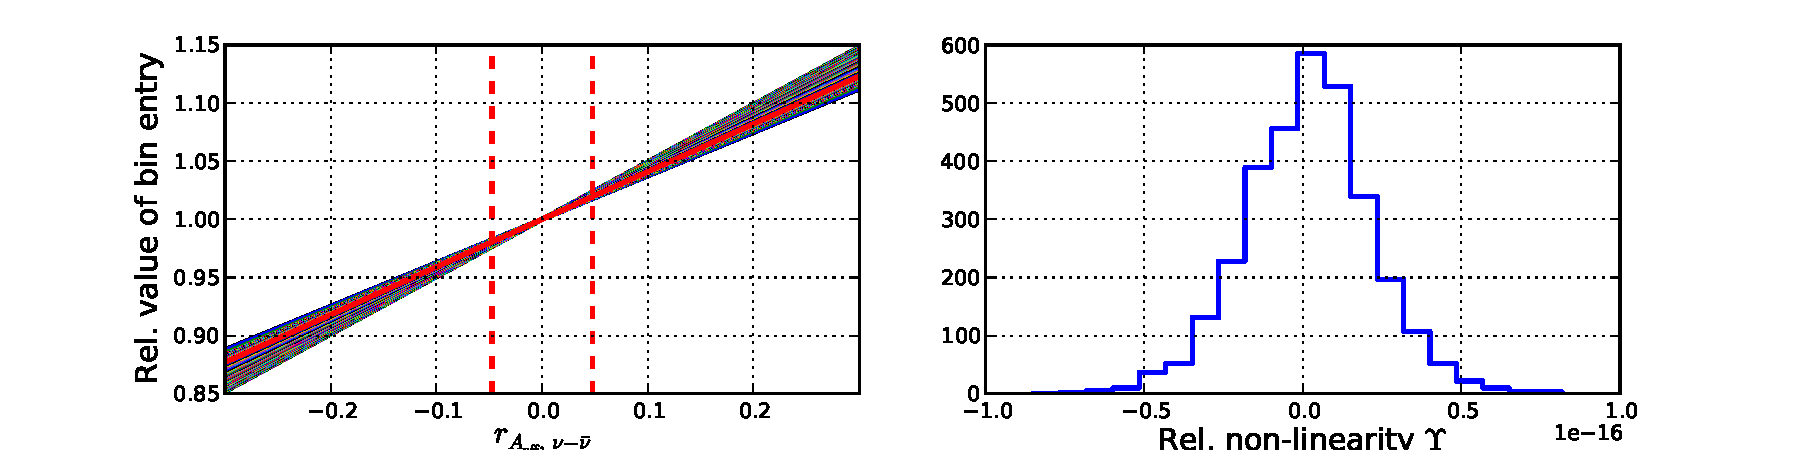
\includegraphics[width=\linewidth]{nu_rel_xsec_scale}
 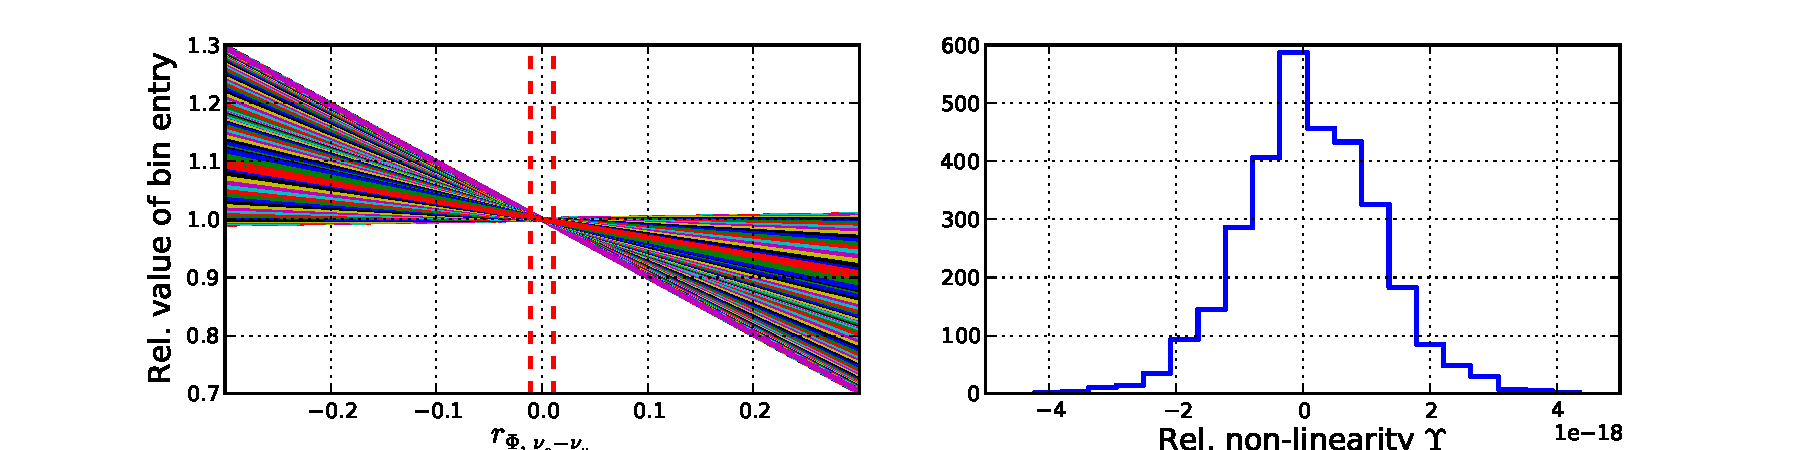
\includegraphics[width=\linewidth]{nue_numu_flux_scale}
 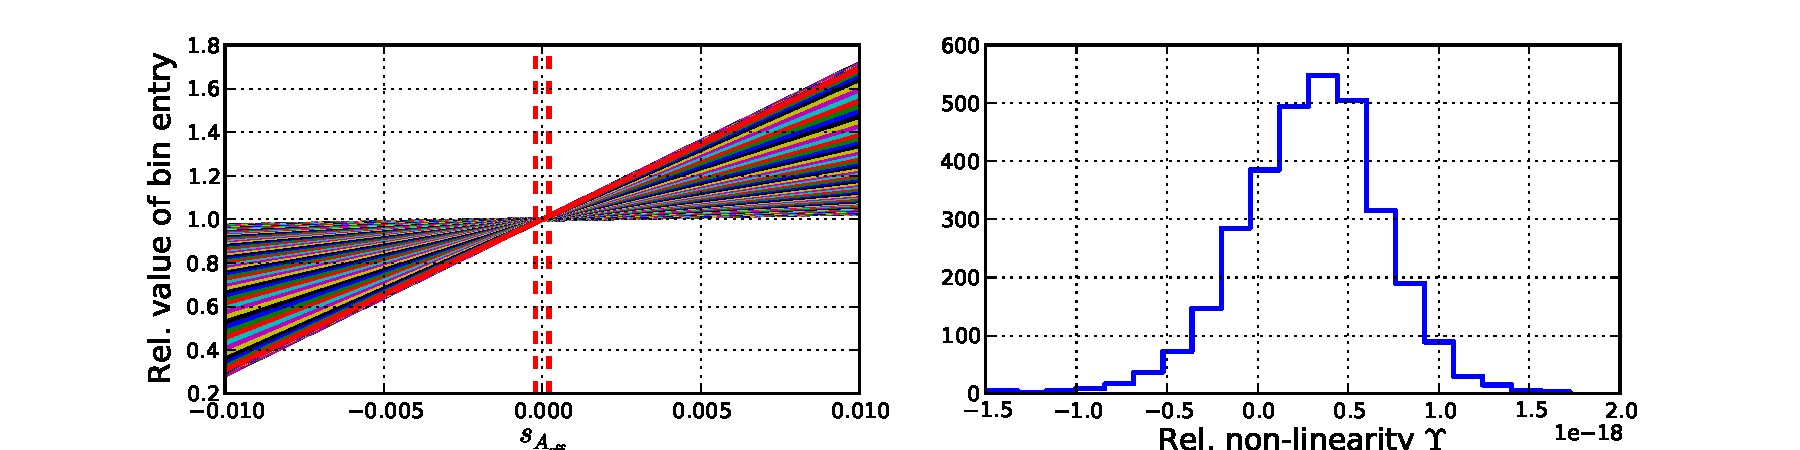
\includegraphics[width=\linewidth]{a_eff_scale}
 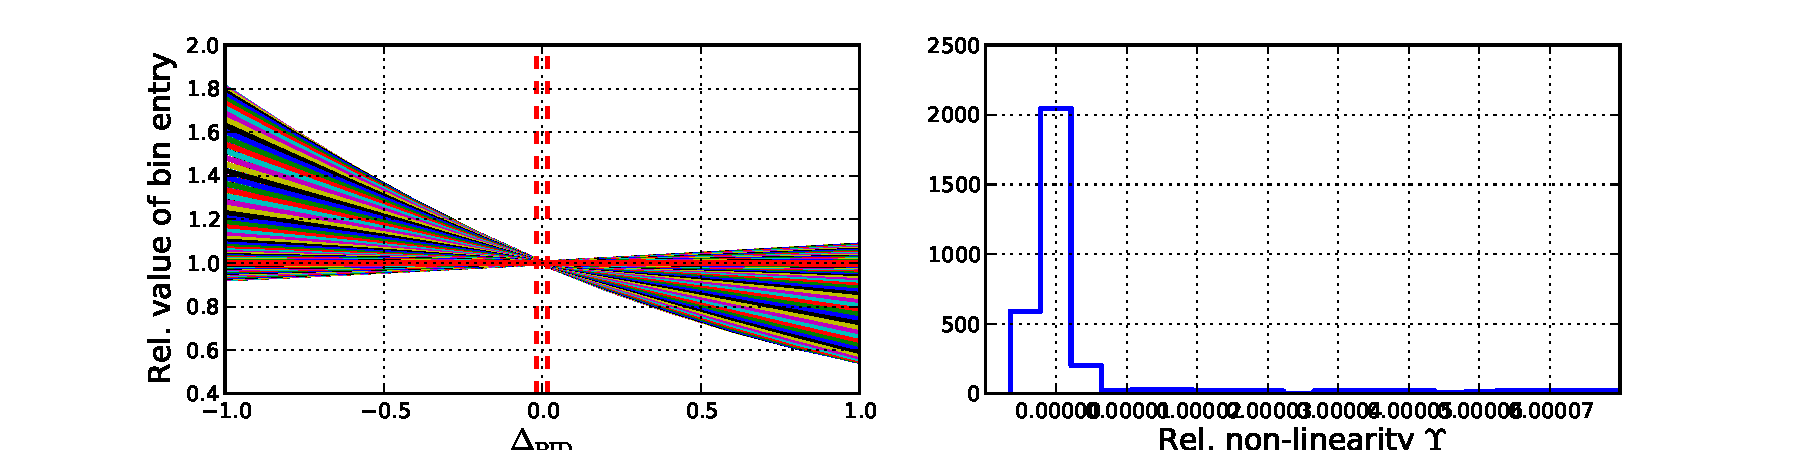
\includegraphics[width=\linewidth]{PID_offset}
 \caption{Same as Fig.~\ref{fig:nonlinearities1} for the remaining parameters.}
 \label{fig:nonlinearities2}
\end{figure}


\chapter{Oscillation Probabilities}
\label{app:oscillation}

\begin{figure}[h]
 \centering
 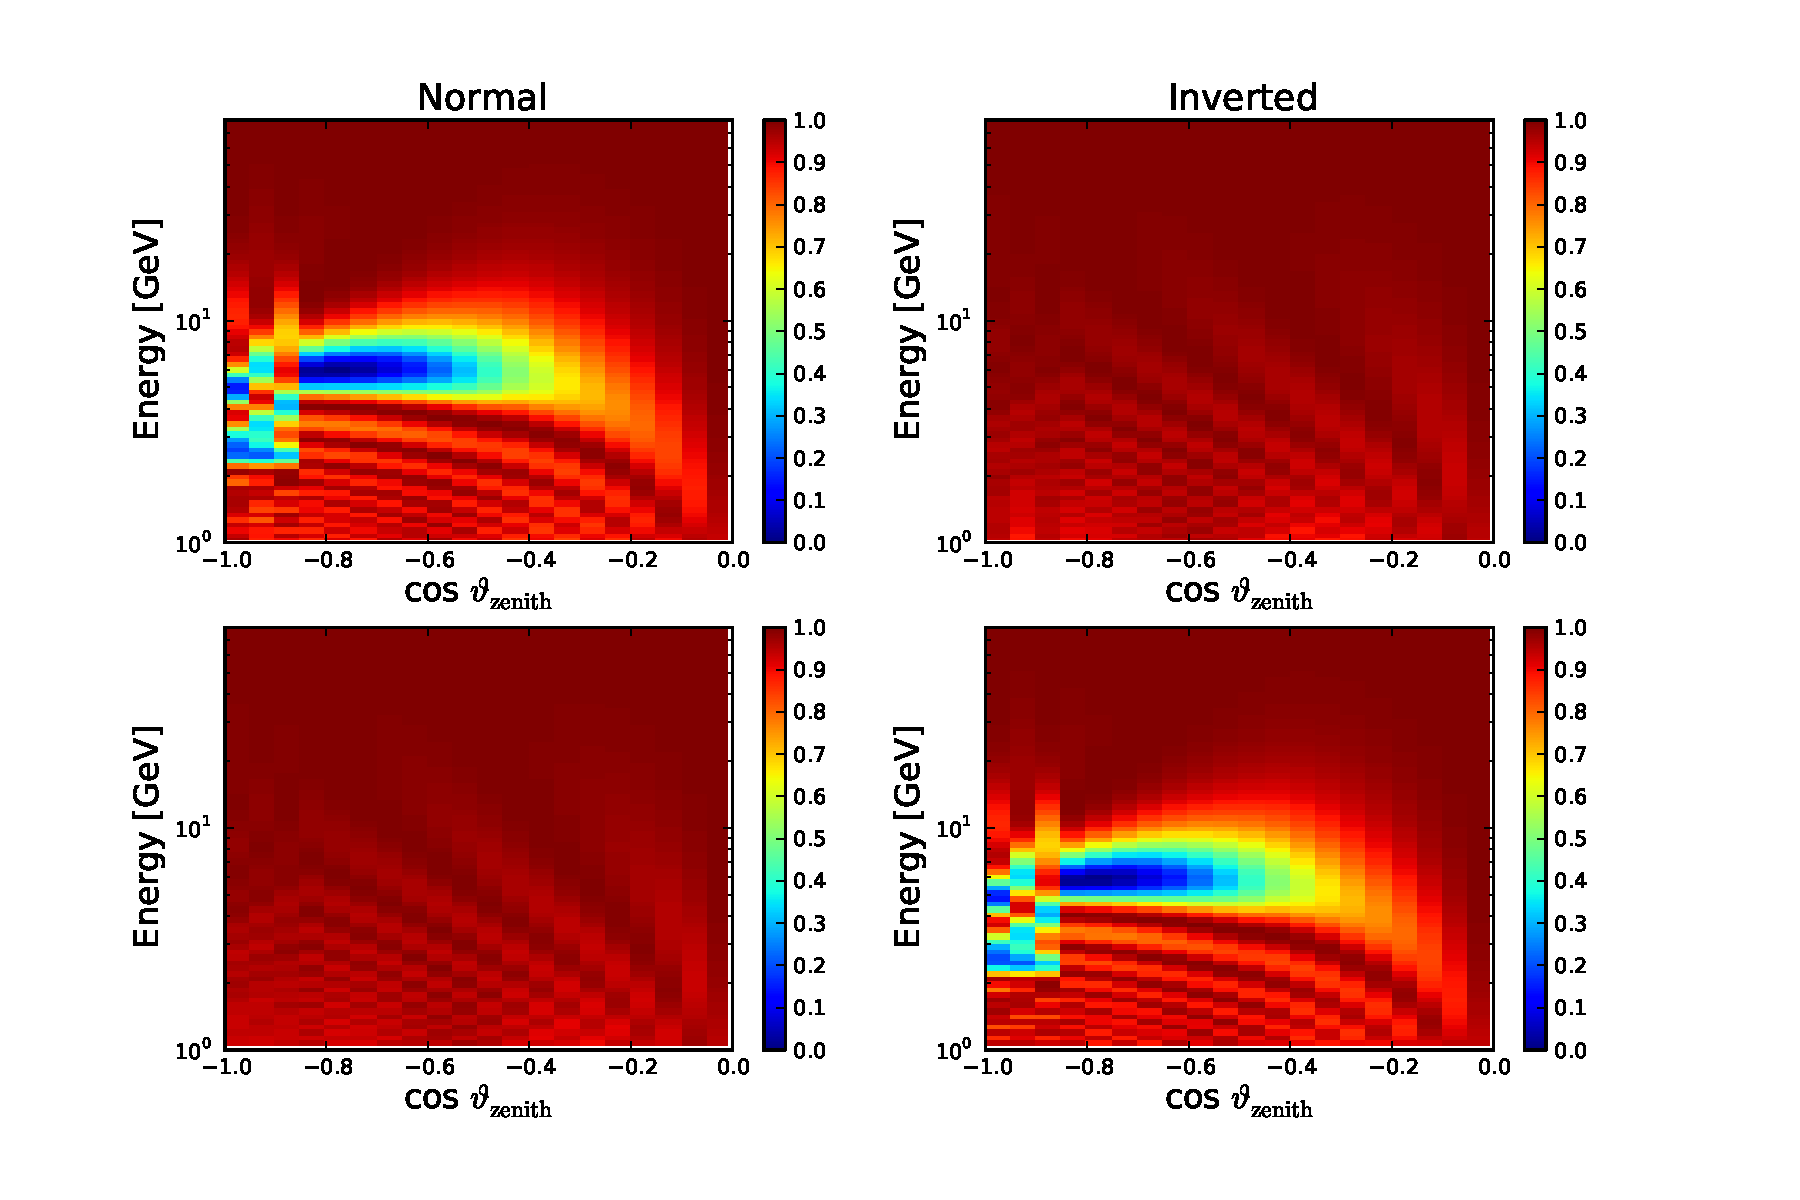
\includegraphics[width=0.95\textwidth]{osc_ds_nue_to_nue}
 \caption{Oscillation probabilities for $\nue \to \nue$ (top) and $\nuebar \to
          \nuebar$ (bottom) for normal and inverted hierarchy.}
\end{figure}


\begin{figure}[t!]
 \centering
 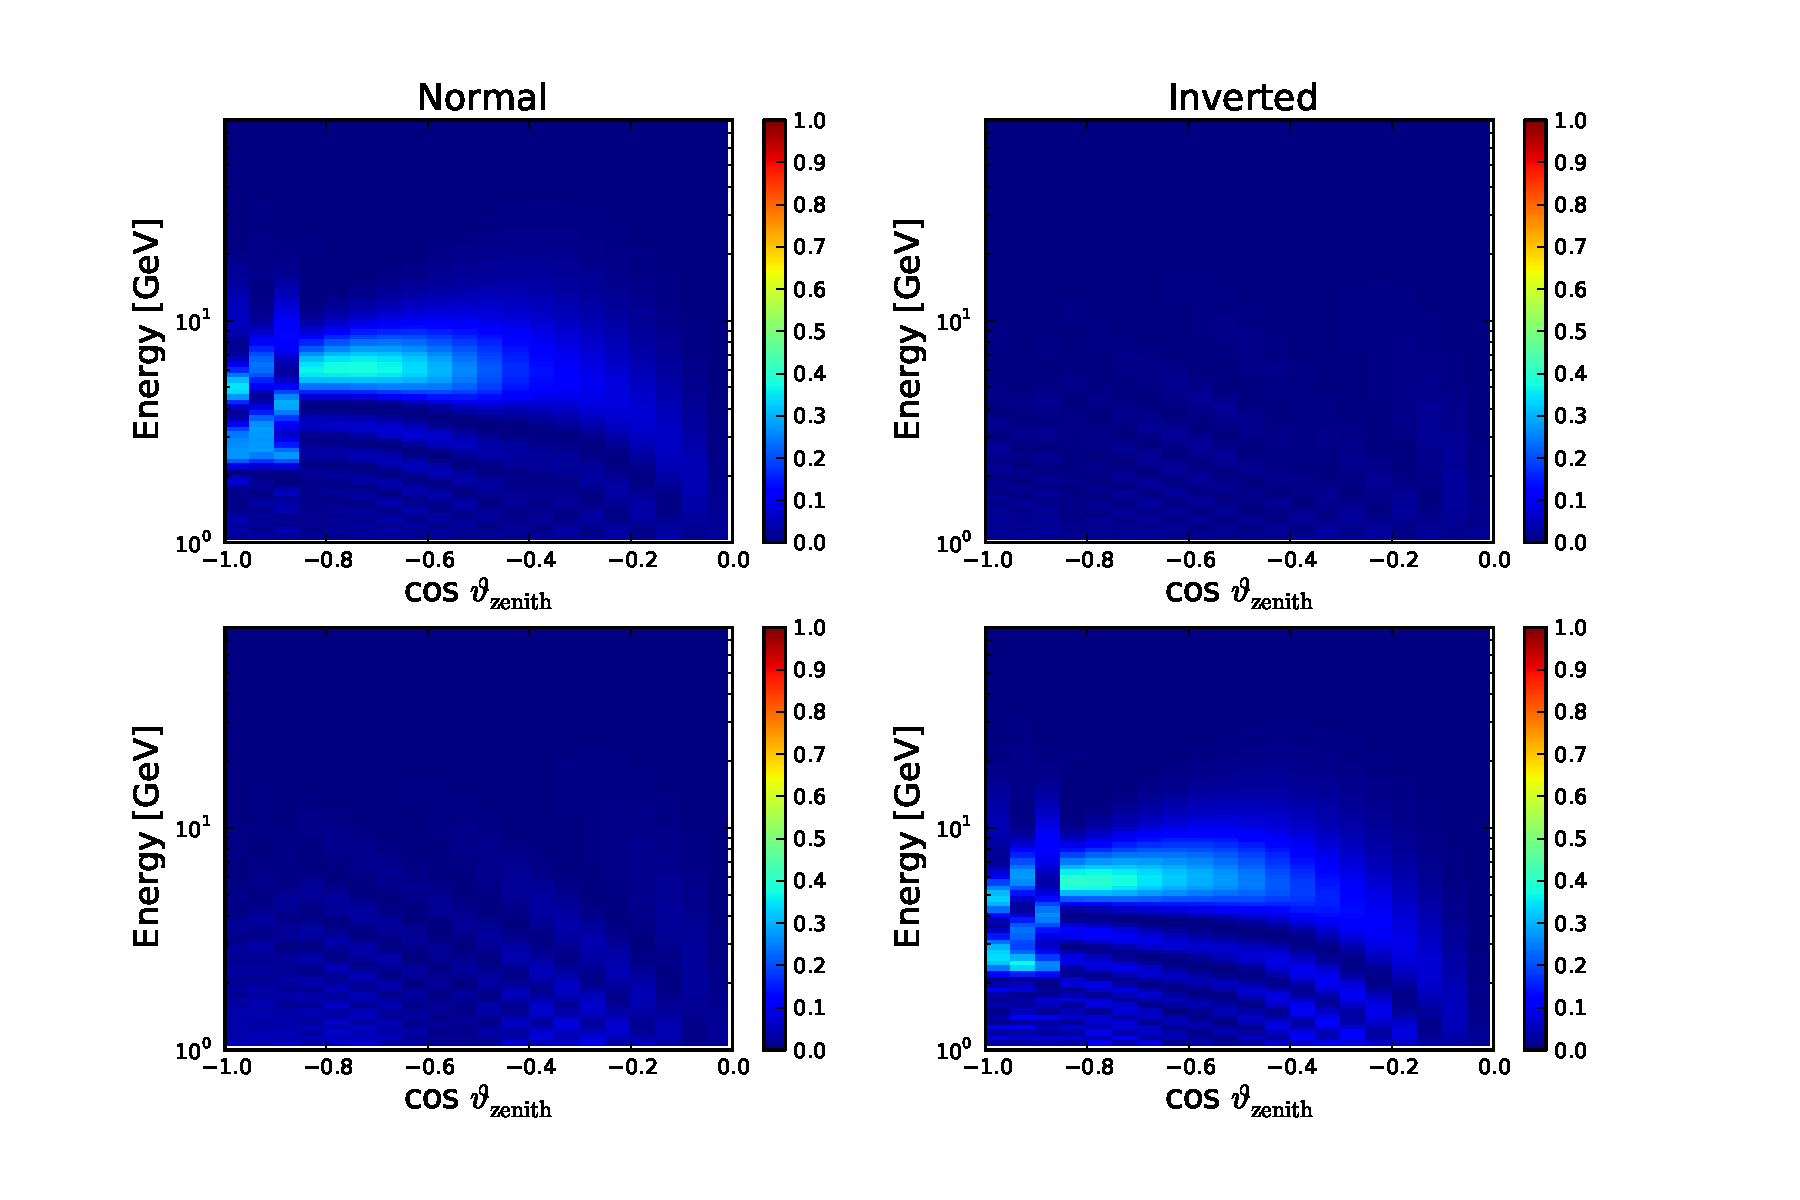
\includegraphics[width=0.95\textwidth]{osc_ds_nue_to_numu}
 \caption{Oscillation probabilities for $\nue \to \numu$ (top) and $\nuebar \to
          \numubar$ (bottom) for normal and inverted hierarchy.}
\end{figure}

\begin{figure}[b!]
 \centering
 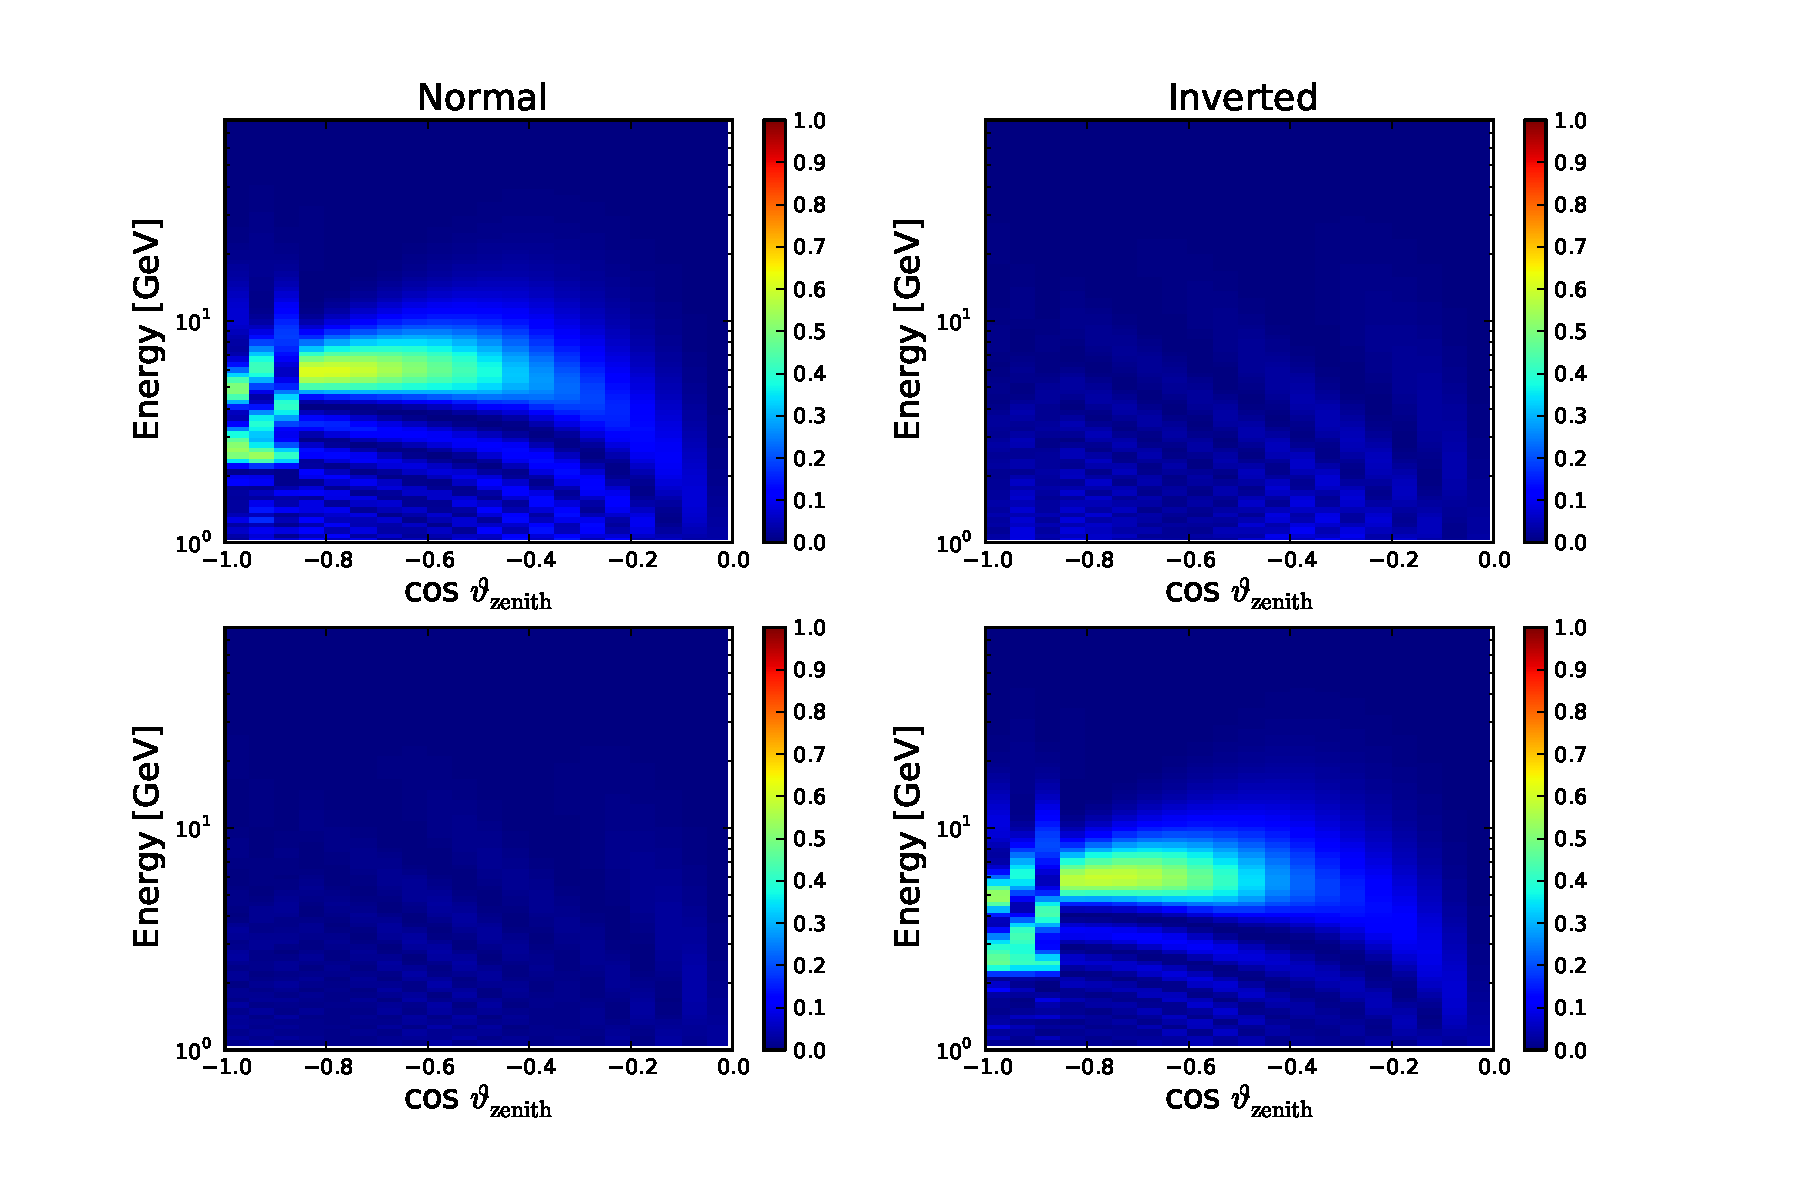
\includegraphics[width=0.95\textwidth]{osc_ds_nue_to_nutau}
 \caption{Oscillation probabilities for $\nue \to \nutau$ (top) and $\nuebar \to
          \nutaubar$ (bottom) for normal and inverted hierarchy.}
\end{figure}

\begin{figure}[t!]
 \centering
 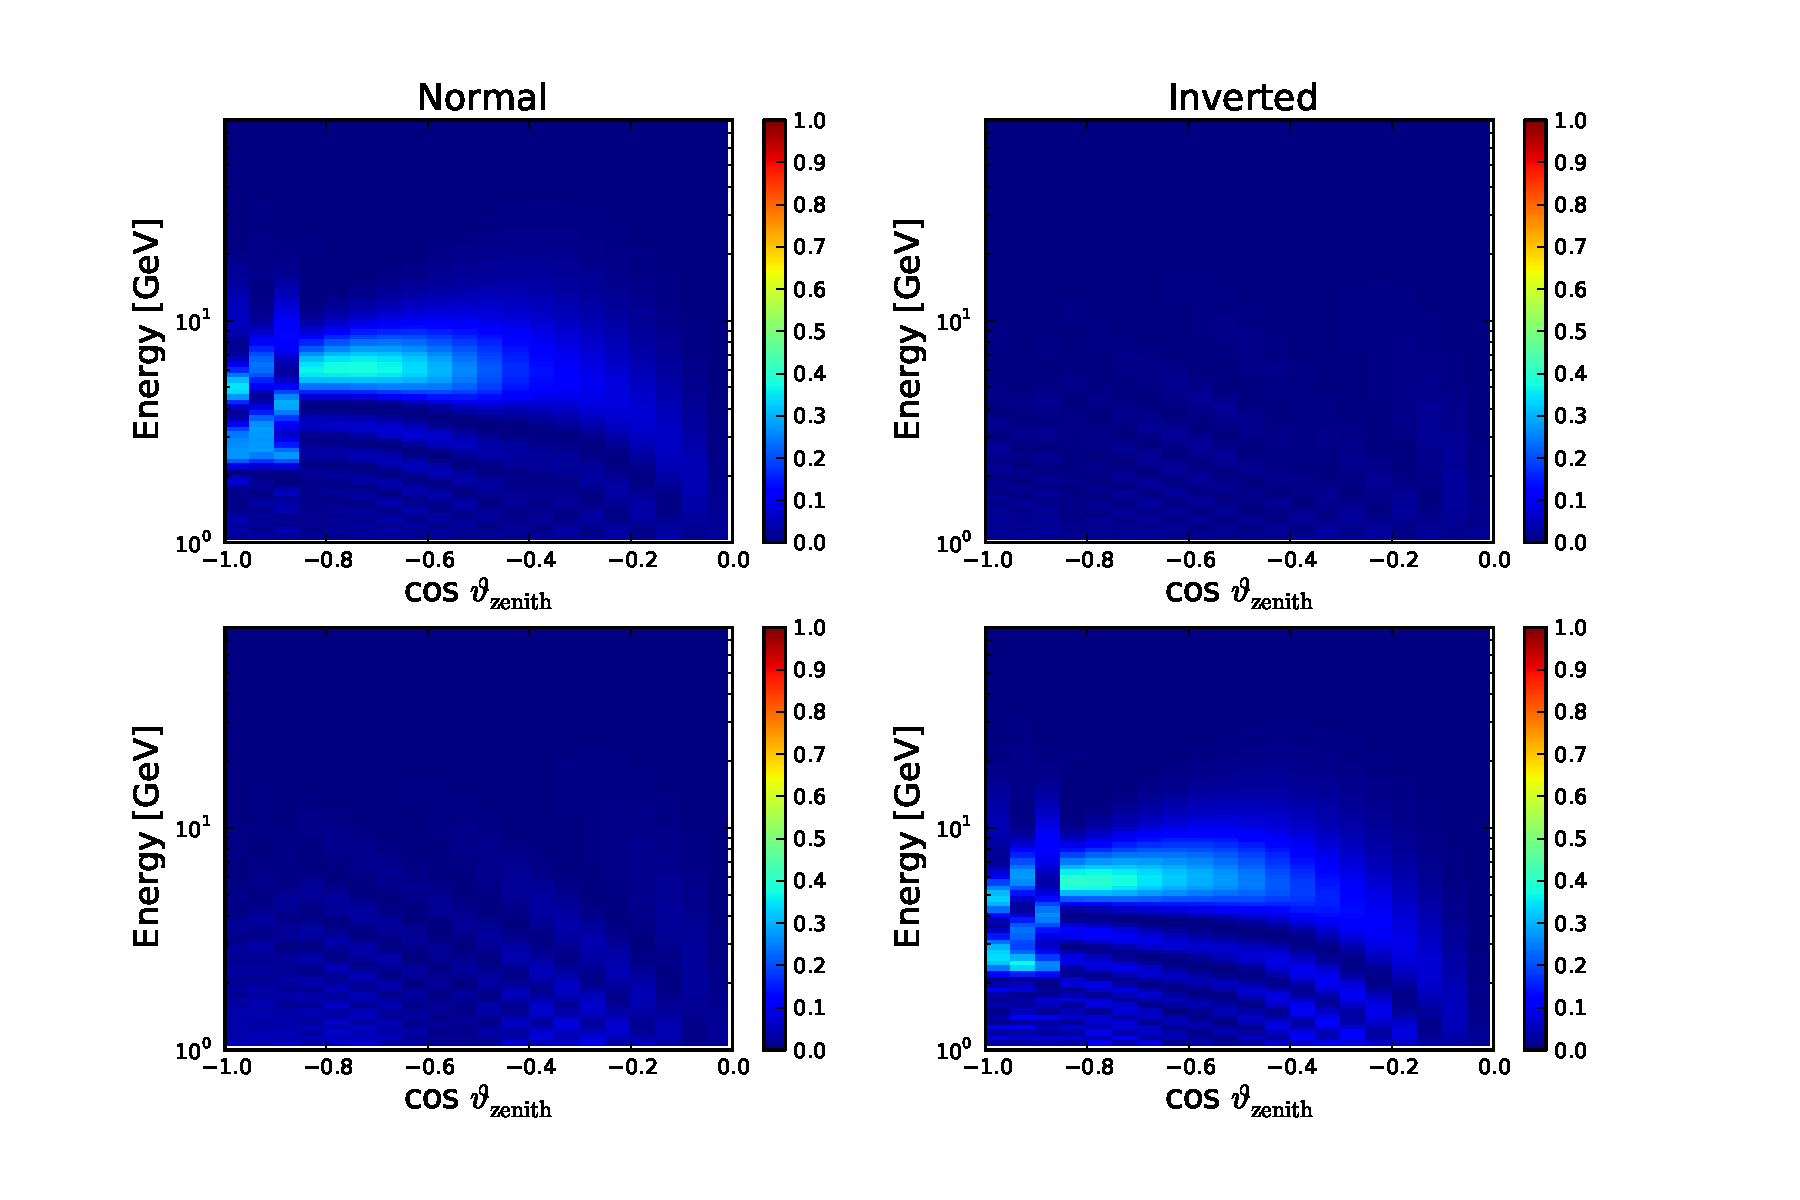
\includegraphics[width=0.95\textwidth]{osc_ds_numu_to_nue}
 \caption{Oscillation probabilities for $\numu \to \nue$ (top) and $\numubar \to
          \nuebar$ (bottom) for normal and inverted hierarchy.}
\end{figure}

\begin{figure}[b!]
 \centering
 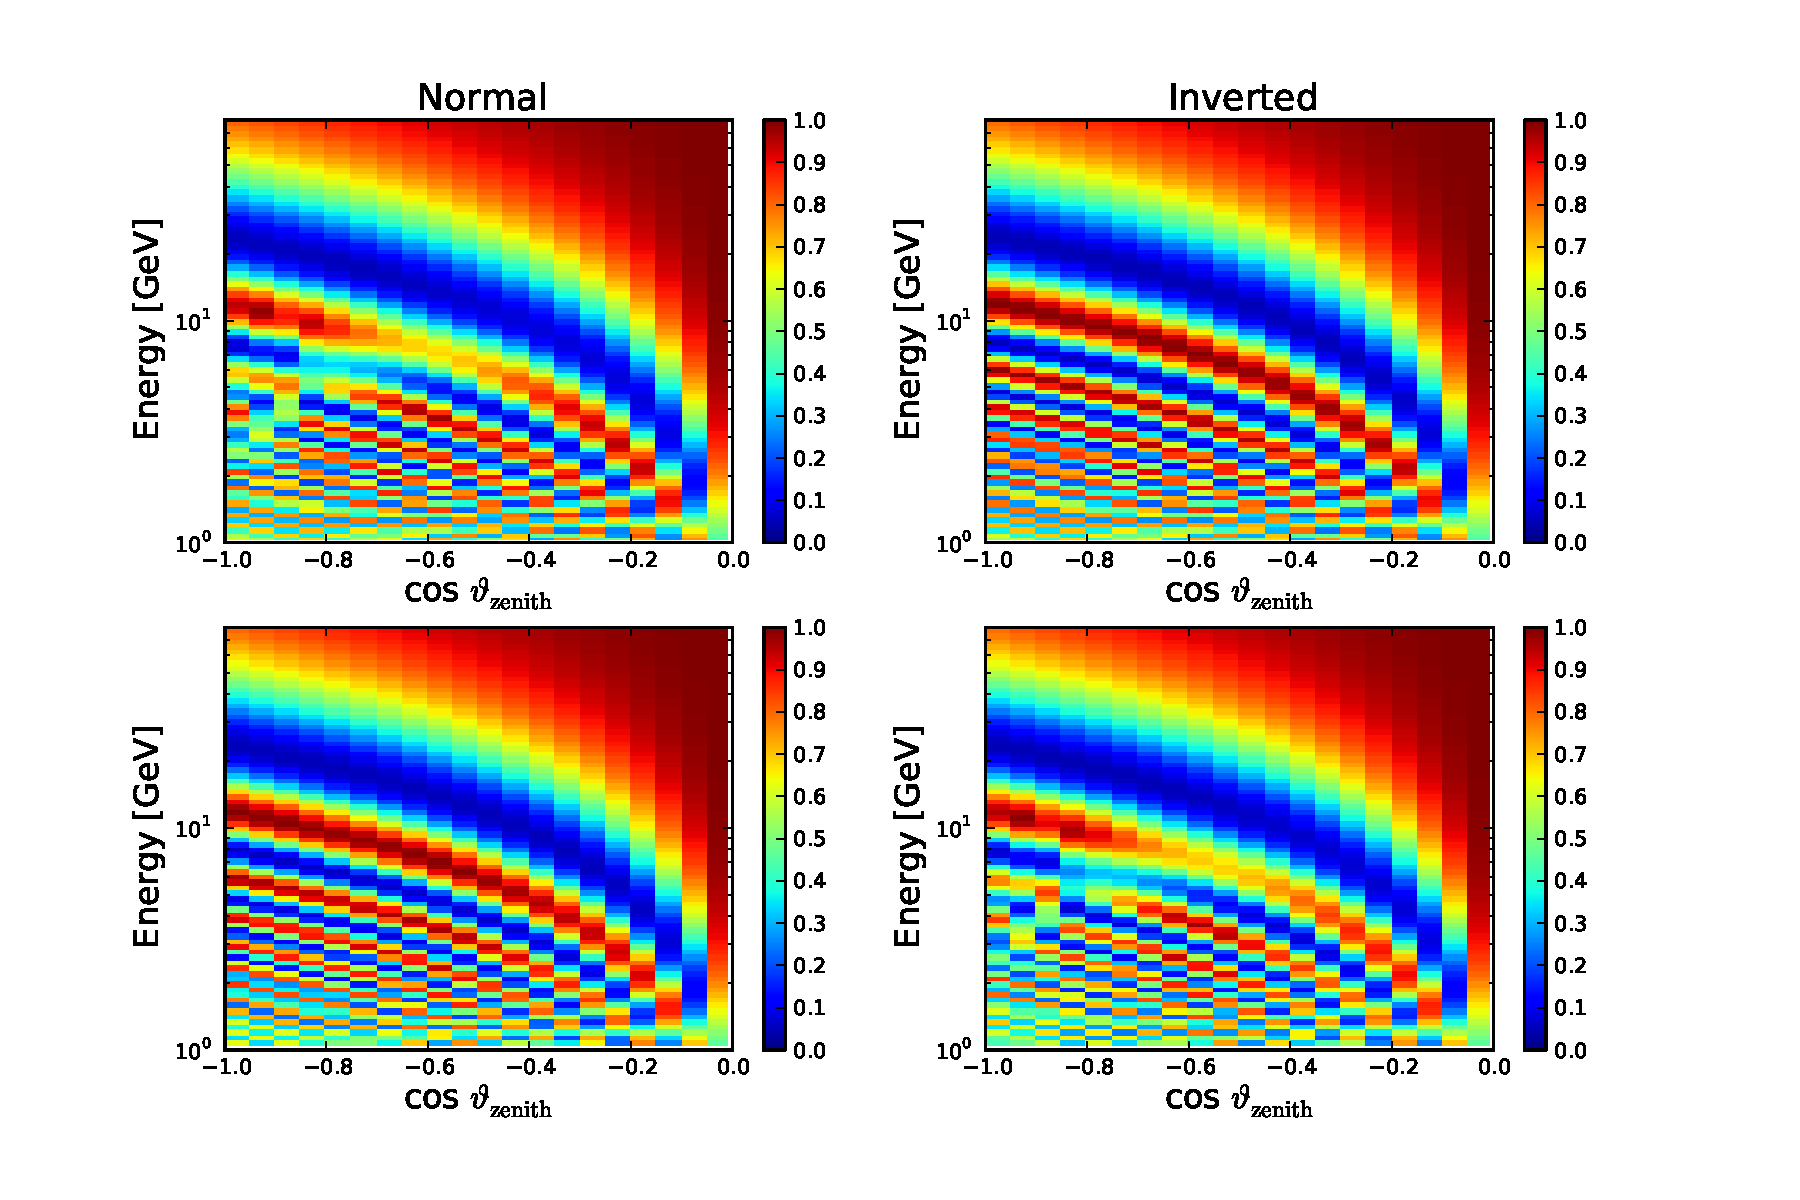
\includegraphics[width=0.95\textwidth]{osc_ds_numu_to_numu}
 \caption{Oscillation probabilities for $\numu \to \numu$ (top) and $\numubar
          \to \numubar$ (bottom) for normal and inverted hierarchy.}
\end{figure}


\begin{figure}[t!]
 \centering
 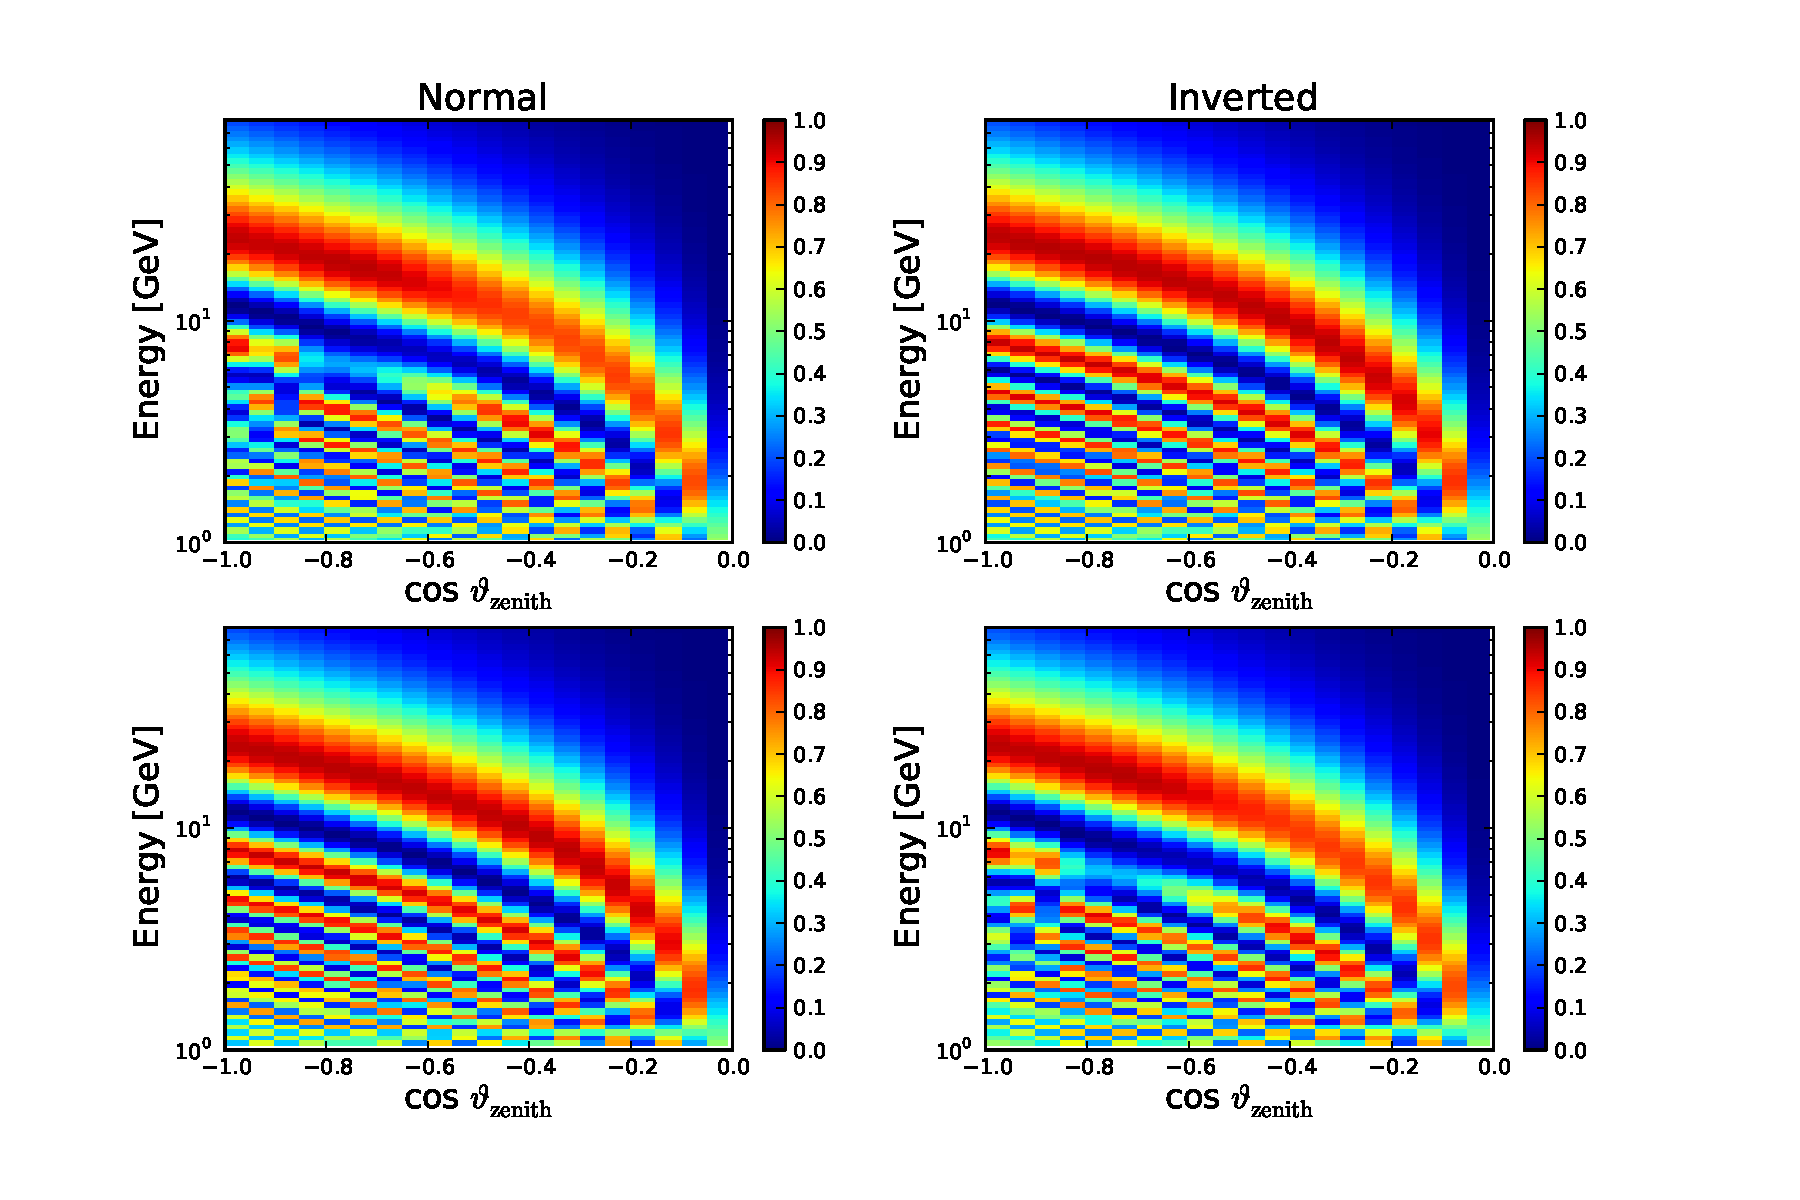
\includegraphics[width=0.95\textwidth]{osc_ds_numu_to_nutau}
 \caption{Oscillation probabilities for $\numu \to \nutau$ (top) and $\numubar
          \to \nutaubar$ (bottom) for normal and inverted hierarchy.}
\end{figure}

\chapter{Parametrisations of the Detector Resolutions}
\label{app:reco_params}

The full parametrisations of the reconstruction performances will be listed in
form of the actual \papa input. These are nested dictionaries giving the
resolutions in energy (\texttt{'e'}) and \coszen (\texttt{'coszen'}) for all
four interaction channels: \nue, \numu, and \nutau CC (\texttt{'nue'},
\texttt{'numu'}, and \texttt{'nutau'}, respectively) and \nux NC
(\texttt{'NC'}). For each of those the resolution is given by the five
parameters \texttt{'fraction'}, \texttt{'loc1'}, \texttt{'loc2'},
\texttt{'width1'}, and \texttt{'width2'}, corresponding to $f$, $\mu_1$,
$\mu_2$, $\sigma_1$ and $\sigma_2$ in (\ref{eqn:reco_param}).

The actual function definitions for the five parameters is then supplied as a
text string that can be interpreted as a python function by python's
\texttt{eval()} function. In those definitions, \texttt{'n'} is a shorthand
for the numpy library \cite{numpy} used for most of the numerical operations in
\papa.

\section{Baseline Settings}

\VerbatimInput{figs/reco_param/reco_default.json}

% \section{Energy Resolution}
% 
% \section{\coszen Resolution}


\chapter{PID Functions}
\label{app:pid}

\section{Baseline Settings}

The particle identification is a binary decision, thus only the track
identification probabilities $P_{\mathrm{channel} \to \mathrm{track}}$ are
listed:
\begin{eqnarray}
 P_{\nue\to\mathrm{track}}(E) =
   0.192 \gauss{\log_{10}(E[\mathrm{GeV}])}{0.878}{0.404} + 0.0309 \\
 P_{\numu\to\mathrm{track}}(E) =
   \frac{0.687}{\stepfunc{\log_{10}(E[\mathrm{GeV}])}{0.683}{0.183}} + 0.0585 \\
 P_{\nutau\to\mathrm{track}}(E) =
   0.197 \gauss{\log_{10}(E[\mathrm{GeV}])}{1.28}{0.466} + 0.0732 \\
 P_{\nux\,\mathrm{NC}\to\mathrm{track}}(E) =
   0.171 \gauss{\log_{10}(E[\mathrm{GeV}])}{1.37}{0.483} + 0.0339
\end{eqnarray}
The cascade identification probabilities are given by $P_{\mathrm{channel} \to
\mathrm{cascade}} = 1 - P_{\mathrm{channel} \to \mathrm{track}}$.


\chapter{Full Error Listings}
\label{app:fisher_output}

Here the full error lists, similar to Tab.~\ref{tab:baseline_results}, for
various detector settings and sub-channels will be collected. These have
not been included in the main text for the sake of better readability. For a
description how to read the tables, refer to the explanations given for
Tab.~\ref{tab:baseline_results} in Sec.~\ref{sec:results_baseline}.

\section{Baseline Settings}
\label{app:fisher_baseline}

\begin{table}[htpb]
 \caption{Same as Tab.~\ref{tab:baseline_results}, but for the cascade channel
  only}
 \begin{center}
  \small{\begin{tabular}{lrrrrrr} 
\toprule
Parameter & Impact [\%] & Best Fit & $\sigma^\mathrm{full}$ & $\sigma^\mathrm{stat}$ & $\sigma^\mathrm{syst}$ & Prior \\ 
\midrule
$h$ & 100.0 & \num{1.00e+00} & \num{5.17e-01} & \num{3.39e-01} & \num{3.91e-01} & free \\
$r_{\Phi,\,\nu_e-\nu_\mu}$ & 24.9 & \num{0.00e+00} & \num{2.44e-02} & \num{1.06e-02} & \num{2.58e-02} & \num{5.00e-02} \\
$\vartheta_{23}$ [$^\circ$] & 20.7 & \num{3.86e+01} & \num{1.05e+00} & \num{5.78e-01} & \num{1.61e+00} & \num{1.32e+00} \\
$\Delta_\mathrm{PID}$ [GeV] & 11.4 & \num{0.00e+00} & \num{1.53e-01} & \num{4.14e-02} & \num{1.55e-01} & \num{5.00e-01} \\
$s_{A_\mathrm{eff}}$ [m$^2$/GeV] & 4.5 & \num{0.00e+00} & \num{3.96e-04} & \num{1.85e-04} & \num{3.50e-04} & free \\
$r_{A_\mathrm{eff},\,\nu-\bar\nu}$ & 4.2 & \num{0.00e+00} & \num{4.91e-02} & \num{5.55e-03} & \num{2.60e-01} & \num{5.00e-02} \\
$\vartheta_{13}$ [$^\circ$] & 3.0 & \num{8.93e+00} & \num{4.66e-01} & \num{1.67e+00} & \num{5.53e+00} & \num{4.68e-01} \\
$s_E$ & 1.5 & \num{1.00e+00} & \num{3.14e-02} & \num{1.92e-02} & \num{3.55e-02} & \num{5.00e-02} \\
$\Delta m^2_{31}$ [eV$^2$] & 1.2 & \num{2.46e-03} & \num{6.73e-05} & \num{4.44e-05} & \num{1.16e-04} & \num{8.00e-05} \\
$n_{A_\mathrm{eff}}$ & 0.1 & \num{0.00e+00} & \num{2.29e-02} & \num{2.32e-03} & \num{2.29e-02} & \num{2.00e-01} \\
\bottomrule 
\end{tabular}
}
 \end{center}
\end{table}

\begin{table}[htpb]
 \caption{Same as Tab.~\ref{tab:baseline_results}, but for the track channel
  only}
 \begin{center}
  \small{\begin{tabular}{lrrrrrr} 
\toprule
Parameter & Impact [\%] & Best Fit & $\sigma^\mathrm{full}$ & $\sigma^\mathrm{stat}$ & $\sigma^\mathrm{syst}$ & Prior \\ 
\midrule
$h$ & 100.0 & \num{1.00e+00} & \num{7.47e-01} & \num{3.20e-01} & \num{6.75e-01} & free \\
$s_E$ & 8.4 & \num{1.00e+00} & \num{2.98e-02} & \num{8.36e-03} & \num{3.62e-02} & \num{5.00e-02} \\
$\Delta m^2_{31}$ [eV$^2$] & 7.2 & \num{2.46e-03} & \num{6.70e-05} & \num{1.93e-05} & \num{1.21e-04} & \num{8.00e-05} \\
$\vartheta_{23}$ [$^\circ$] & 5.9 & \num{3.86e+01} & \num{5.83e-01} & \num{3.55e-01} & \num{5.44e-01} & \num{1.32e+00} \\
$\vartheta_{13}$ [$^\circ$] & 3.6 & \num{8.93e+00} & \num{4.67e-01} & \num{9.47e-01} & \num{1.01e+01} & \num{4.68e-01} \\
$r_{\Phi,\,\nu_e-\nu_\mu}$ & 2.4 & \num{0.00e+00} & \num{3.61e-02} & \num{5.84e-03} & \num{5.17e-02} & \num{5.00e-02} \\
$\Delta_\mathrm{PID}$ [GeV] & 2.3 & \num{0.00e+00} & \num{3.82e-02} & \num{1.71e-02} & \num{3.43e-02} & \num{5.00e-01} \\
$s_\mathrm{PID}$ & 1.3 & \num{1.00e+00} & \num{3.04e-02} & \num{3.87e-03} & \num{3.01e-02} & free \\
$s_{A_\mathrm{eff}}$ [m$^2$/GeV] & 0.3 & \num{0.00e+00} & \num{4.13e-04} & \num{1.64e-04} & \num{3.79e-04} & free \\
$r_{A_\mathrm{eff},\,\nu-\bar\nu}$ & 0.2 & \num{0.00e+00} & \num{4.88e-02} & \num{9.29e-03} & \num{2.22e-01} & \num{5.00e-02} \\
\bottomrule 
\end{tabular}
}
 \end{center}
\end{table}
